\XtoCBlock{Not}
\label{block:Not}
\begin{figure}[H]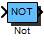
\includegraphics{Not}\end{figure} 

\begin{XtoCtabular}{Inports}
In & \tabularnewline
\hline
\end{XtoCtabular}


\begin{XtoCtabular}{Outports}
Out & \tabularnewline
\hline
\end{XtoCtabular}

\subsubsection*{Description:}
Logical inverter block.

\subsubsection*{Implementations:}
\begin{tabular}{l l}
\textbf{FiP8} & 8 Bit Fixed Point Implementation\tabularnewline
\textbf{FiP16} & 16 Bit Fixed Point Implementation\tabularnewline
\textbf{FiP32} & 32 Bit Fixed Point Implementation\tabularnewline
\end{tabular}

\XtoCImplementation{FiP8}
\index{Block ID!224}
\nopagebreak[0]
% Implementation details
\begin{tabular}{l l}
\textbf{Name} & FiP8 \tabularnewline
\textbf{ID} & 224 \tabularnewline
\textbf{Revision} & 0.1 \tabularnewline
\textbf{C filename} & Not\_FiP8.c \tabularnewline
\textbf{H filename} & Not\_FiP8.h \tabularnewline
\end{tabular}
\vspace{1ex}

8 Bit Fixed Point Implementation

% Implementation data structure
\XtoCDataStruct{Data Structure:}
\begin{lstlisting}
typedef struct {
     uint16        ID;
     int8          *In;
     int8          Out;
} NOT_FIP8;
\end{lstlisting}

\ifdefined \AddTestReports
\InputIfFileExists{\XcHomePath/Library/General/Doc/Test_Not_FiP8.tex}{}{}
\fi
\XtoCImplementation{FiP16}
\index{Block ID!225}
\nopagebreak[0]
% Implementation details
\begin{tabular}{l l}
\textbf{Name} & FiP16 \tabularnewline
\textbf{ID} & 225 \tabularnewline
\textbf{Revision} & 0.1 \tabularnewline
\textbf{C filename} & Not\_FiP16.c \tabularnewline
\textbf{H filename} & Not\_FiP16.h \tabularnewline
\end{tabular}
\vspace{1ex}

16 Bit Fixed Point Implementation

% Implementation data structure
\XtoCDataStruct{Data Structure:}
\begin{lstlisting}
typedef struct {
     uint16        ID;
     int16         *In;
     int16         Out;
} NOT_FIP16;
\end{lstlisting}

\ifdefined \AddTestReports
\InputIfFileExists{\XcHomePath/Library/General/Doc/Test_Not_FiP16.tex}{}{}
\fi
\XtoCImplementation{FiP32}
\index{Block ID!226}
\nopagebreak[0]
% Implementation details
\begin{tabular}{l l}
\textbf{Name} & FiP32 \tabularnewline
\textbf{ID} & 226 \tabularnewline
\textbf{Revision} & 0.1 \tabularnewline
\textbf{C filename} & Not\_FiP32.c \tabularnewline
\textbf{H filename} & Not\_FiP32.h \tabularnewline
\end{tabular}
\vspace{1ex}

32 Bit Fixed Point Implementation

% Implementation data structure
\XtoCDataStruct{Data Structure:}
\begin{lstlisting}
typedef struct {
     uint16        ID;
     int32         *In;
     int32         Out;
} NOT_FIP32;
\end{lstlisting}

\ifdefined \AddTestReports
\InputIfFileExists{\XcHomePath/Library/General/Doc/Test_Not_FiP32.tex}{}{}
\fi
